\chapter{Triaxial Nuclei and Their Signatures}

In the following chapter, some theoretical background that is necessary for understanding triaxiality will be presented, with examples from literature and also some results obtained by this team. It is also instructive to realize why the nuclear community focuses their attention to the highly deformed nuclei, and moreover, nuclei which depart so much from the spherical shapes that they become \emph{triaxial}.

Presenting the theoretical formalism that is used to describe triaxial nuclei, and mention the \emph{fingerprints} of nuclear triaxiality is that last step before diving into the recently developed framework for odd-$A$ nuclei which the team created, and showing the results. 

\section{Non-axial nuclei}

The discussion regarding excitation energies of a rigid rotator from the previous chapter was focused on pure rotators or nuclei with axially symmetric shapes (i.e,, prolate or oblate). Remember that deformation is still required in order to define a collective spectra with rotational character. Moreover, the relevant quantities that are involved in the rotational motion for a deformed nucleus are the moments of inertia corresponding to the principal axes of the deformed ellipsoid: $\mathcal{I}_{1,2,3}$, and within previous calculations, two moments of inertia were supposed to be identical.

Even though calculations are performed with the rigid-like MOI or the irrotational-like, their dependence on the deformation parameters $\beta_2$ and $\gamma$ is present (recall expressions given in Eq. \ref{eq-irrotational-rigid-mois}). Taking a closer look at their evolution with $\gamma$, one can see that indeed, identical MOI can only occur at certain values (see Fig. \ref{fig-irrotational-rigid-mois}). As such, the nuclei can be regarded (when referring to their ground state) as such:
\begin{itemize}
    \item \textbf{Spherical:} all MOI are identical and no deformations are present
    \item \textbf{Axially-symmetric:} two identical MOI and only the $\beta_2$ parameter plays a role in the collective phenomena of these nuclei
    \item \textbf{Triaxial (Axially-asymmetric):} all three MOI are different (usually one of them is very large when compared to the other two), the quadrupole deformation parameter as well as the triaxiality parameter $\gamma$ are present
\end{itemize}

Now, across the chart of nuclides, most of the isotopes are either spherical either symmetric in their ground state \cite{budaca2018tilted}, but triaxial shapes might also occur as ground-state \cite{moller2006global}. The apparition of triaxial nuclei implies some kind of `stability' on the $\gamma$-parameter, since a dynamical character of the triaxiality will indicate some transitional states rather than nuclear stability. Indeed, a rigid (fixed) value for $\gamma$ is required around the minimal region of the potential energy surface such that triaxial stable nuclei can exist. Thus, one can distinguish between the $\gamma$-soft nuclei in which this parameter has a dynamical character and the $\gamma$-rigid ones, which could in fact exhibit stable triaxial deformation \cite{dracoulis2013isomers}.
Even more interesting are the structures which occur at very large values of quadrupole deformation $\beta_2$ and $\gamma$ in the vicinity of $\approx 30^\circ$ (where maximal triaxiality occurs). It will be shown that these last nuclei will lead to band structures that are called \emph{Triaxial Strongly Deformed} bands (TSD for short) \cite{odegaard2001evidence,jensen2002evidence}.

Concluding, the triaxial nuclei are a special class of nuclei in which there is an asymmetry between the moments of inertia (given by a $\gamma$ value within the corresponding interval), and moreover, the quadrupole deformation is high enough such that it stabilizes the entire system.

\subsection{Triaxial Rotor Model}

The most general Hamiltonian for a \emph{triaxial system} is given in terms of the components of the total angular momentum operator $\hat{I}$ and the moments of inertia for the deformed ellipsoid, similarly as it was the case for the \emph{rotational Hamiltonian} within the symmetry case:
\begin{align}
    \hat{H}=\frac{\hat{I}_1^2}{2\mathcal{I}_1}+\frac{\hat{I}_2^2}{2\mathcal{I}_2}+\frac{\hat{I}_3^2}{2\mathcal{I}_3}\ ,
\end{align}
where the indices correspond to each of the principal axes of the rotational ellipsoid (principal axes are the ones in which the components of the MOI tensor are diagonal). More often, the notations $A_{1,2,3}=\frac{\hbar^2}{2\mathcal{I}_{1,2,3}}$ are used in the Hamiltonian's expression, leading to $A_1\neq A_2\neq A_3$ for the triaxial nuclei. Shi et al. \cite{wen2015wobbling} show a very straightforward way of obtaining the eigenvalues for the \emph{triaxial rigid rotor}, following the quantum treatment made by Davydov and Filippov for the rigid rotor without symmetry axis \cite{davydov1958rotational}:
\begin{align}
    \hat{H}&=\hat{H}_\text{diag}+\hat{H}_\text{non-diag}\ ,\nonumber\\
    \hat{H}_\text{diag}&=\left[\frac{1}{2}\left(A_1+A_2\right)\left(\hat{I}^2-\hat{I}_3^2\right)+A_3\hat{I}_3^2\right]\ ,\nonumber\\
    \hat{H}_\text{non-diag}&=\frac{1}{4}\left(A_1-A_2\right)\left(\hat{I}_+^2+\hat{I}_-^2\right)\ .
\end{align}
This way of expressing the Hamiltonian is useful because there is a clear difference between a term which is diagonal and one that mixes states with different $\Delta K=\pm2$ quantum number. It is important to emphasize that this kind of Hamiltonian is still invariant to rotations with $\pi$ around the principal axes. This is useful because one can solve the eigenvalue problem with the basis $\ket{IMK}$, were the wave-function is described as:
\begin{align}
    \ket{IMK}=\sqrt{\frac{2I+1}{16\pi^2(1+\delta_{K0})}}\left[\ket{IMK}+(-)^I\ket{IM-K}\right]\ ,
\end{align}
where $\ket{IM\pm K}$ are the Wigner $D_{MK}^I$ - functions that determine the \emph{orientation} of the nucleus itself (their are functions of the three Euler angles), the $K$ quantum number is the projection of $I$ onto the 3-axis of the body-fixed frame (intrinsic frame of reference), and the $M$ number represents the projection of $I$ onto the $z$-axis of the laboratory frame. This wave-function is quite similar to the one defined in Eq. \ref{RAL-bands-wave-function}, when the decoupled states in the Rotation Aligned Bands were studied. Indeed, using this basis, the total Hamiltonian can be diagonalized \cite{wen2015wobbling} as such:
\begin{align}
    \hat{H}_{IK}=\frac{1}{2}(A_1+A_2)\left[I(I+1)-K^2\right]+A_3K^2\ ,
\end{align}
with the notation $H_{IK}\equiv\bra{IK}\hat{H}\ket{IK}$. The second, non-diagonal term will have the energy states given as:
\begin{align}
    \hat{H}_{IK\pm2}=\frac{1}{4}(A_1-A_2)\sqrt{(I\mp K)(I\pm K +1)(I \mp K -1)(I\pm K +2)}\ ,
\end{align}
where $\hat{H}_{IK\pm 2}\equiv \bra{IK}\hat{H}\ket{I\pm K}$. Finally, using these matrix elements, the energies can be obtained by solving the eigenvalue equation for given spins $I$. Such calculations were performed by the team for an even-even nucleus $^{158}$Er (see Fig. 8 from  \cite{raduta2017semiclassical}) and the results of the diagonalization procedure were in complete agreement with alternative descriptions for $\hat{H}$.

\subsection{Triaxial Particle + Rotor Model}

In this section, a general discussion about the Hamiltonian for a system which is composed on one single-particle (valence nucleon) in a high-$j$ shell and one triaxial core. Usually, such a treatment will be applied to odd-$A$ triaxial nuclei, and in fact the team's developed framework is founded on the triaxial PRM \cite{davydov1958rotational}. Davydov et al. developed this model for explaining the low-lying collective spectra of $2^+$ states within some transitional nuclei.

The Hamiltonian of this system will be composed of a term which corresponds to the even-even core and that of a single-particle which is moving in a quadrupole deformed mean-field (remember that quadrupole deformation are the only relevant effects when discussing triaxial structures).
\begin{align}
    \hat{H}=\hat{H}_\text{rot}+\hat{H}'_\text{sp}\ .
\end{align}

Here, an important remark must be done regarding the notation of the terms. Usually, the single-particle Hamiltonian is composed of a term that gives the \emph{intrinsic} energy coming from the $j$ shell in which the nucleon is orbiting (one can think of it as representing the Fermi energy level) and a term that characterizes the effective interaction between the particle and the deformed mean-field generated by the core. Consequently, the Hamiltonian $\hat{H}'_\text{sp}$ should be written as: $$\hat{H}'_\text{sp}=\hat{h}_0^j+\hat{H}_\text{int}^\text{quad}\ ,$$where $\hat{h}_0^j$ is the formerly described term and $\hat{H}_\text{int}^\text{quad}$ is the latter.
%the contribution of the total particle energy coming from the position of the $j$-shell and $\hat{H}_\text{int}^\text{quad}$ is the interaction of the valence nucleon with the even-even core (that is of quadrupole type). 
For example, Ring et al. \cite{ring2004nuclear} uses the SHO for describing $\hat{h}_0^j$. The interaction Hamiltonian is in fact a $\gamma$-deformed Nilsson potential, which was previously discussed (see Section \ref{nilsson-model-section}), with it's general expression in this case written as:
\begin{align}
    \hat{H}_\text{int}^\text{quad}=\kappa\beta r^2\left[\cos\gamma Y_{2}^{0}+\frac{\sin\gamma}{\sqrt{2}}\left(Y_2^2+Y_2^{-2}\right)\right].
    \label{quadrupole-deformed-potential-beta}
\end{align}
However, this generalized expression can be written for the single-particle characterized by its total angular momentum $\mathbf{j}$ in the following way:
\begin{align}
    \hat{H}_\text{int}^\text{quad}=\frac{V}{j(j+1)}\left[\cos\gamma(3j_z^2-\mathbf{j}^2)-\sqrt{3}\sin\gamma(j_x^2-j_y^2)\right]\ ,
    \label{single-particle-nilsson-defored-potential}
\end{align}
where the entire interaction strength between the particle and the core is embedded within the value of a parameter (usually adjustable) called \emph{single-particle potential strength} $V$. This parameter is very important in the present research, since the obtained theoretical results regarding energy spectra was obtained through the determination of $V$ numerically.

Peng et al. \cite{peng2003description} gave a description for nuclei within the mass region $A\approx 100,130$ using a Hamiltonian in which two valence nucleons were coupled to the triaxial core (due to the nuclear chirality arising from the odd-odd nature of nuclei). Their Hamiltonian was given as:
\begin{align}
    \hat{H}=\hat{H}_\text{intr}+\hat{H}_{coll}\ ,
\end{align}
where $\hat{H}_\text{coll}$ is the typical rotor Hamiltonian and $\hat{H}_\text{intr}$ represents the sum of a proton and neutron contribution, respectively:
\begin{align}
    \hat{H}_\text{intr}=h_p+h_n\ .
\end{align}
A remarking feature of this approach is that the problem can be extrapolated to a case with multiple protons and neutrons, invoking some sort of `scalability' of their model. Furthermore, the deformed potential (Eq. \ref{quadrupole-deformed-potential-beta}) that gives the energy splittings for the nucleonic orbits (recall the Nilsson diagrams Figs. \ref{nillson-diagram} - \ref{nillson-diagram-2}) is expressed in terms of the nucleus's mass and the quadrupole deformation parameter \cite{peng2003description}:
\begin{align}
    V_\text{int}^\text{quad}=\frac{206}{A^{1/3}}\beta_2\left[\cos\gamma Y_2^0+\frac{\sin\gamma}{\sqrt{2}}(Y_2^2+Y_2^{-2})\right]\ .
    \label{quadrupole-deformed-potential-V}
\end{align}
The single-particle energies for protons and neutrons have a somewhat similar form as the one stated in Eq. \ref{single-particle-nilsson-defored-potential}, namely it is given as:
\begin{align}
    h_p(n)=\pm\frac{1}{2}C_\beta\left[\left(j_3^2-\frac{j(j+1)}{3}\right)\cos\gamma+\frac{1}{2\sqrt{3}}(j_+^2+j_-^2)\sin\gamma\right]\ ,
\end{align}
with the alternating signs corresponding to the proton and neutron, respectively. The \emph{coupling parameter} $C_\beta$ is a measure of energy (typically expressed in MeV units) and its value depends linearly on $\beta$:
\begin{align}
    C_\beta=\frac{195}{j(j+1)}\beta A^{-1/3}\ .
\end{align}
% \subsubsection*{Numerical application - Deformed Potential}
It is worth giving some quantitative results concerning the quadrupole potential and the single-particle Hamiltonian described above. As such, a simple numerical application will be employed, giving graphical representations with the behavior of these quantities with respect to the deformation parameters. Firstly, the potential $V_\text{int}^\text{quad}$ will be analyzed in the polar plane defined by the angles $(\theta,\varphi)$ which enter in the expression of the spherical harmonics. For nuclei within $A\approx 160$ region, it is common to have values of $\beta_2\approx 0.2,0.3$ and $\gamma\approx 20^\circ$, so values for these parameters will be given within this range. The quadrupole potential $V_\text{int}^\text{quad}$ can be seen in Figs. \ref{figs-deformed-quadrupole-potential-1} - \ref{figs-deformed-quadrupole-potential-2}.

\begin{figure}
    \centering
    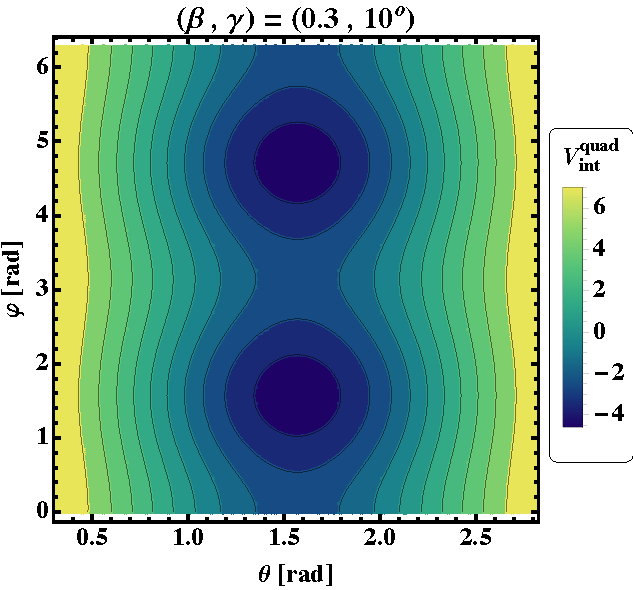
\includegraphics[scale=0.66]{Chapters/Figures/quadrupole-potentialV-1.pdf}
    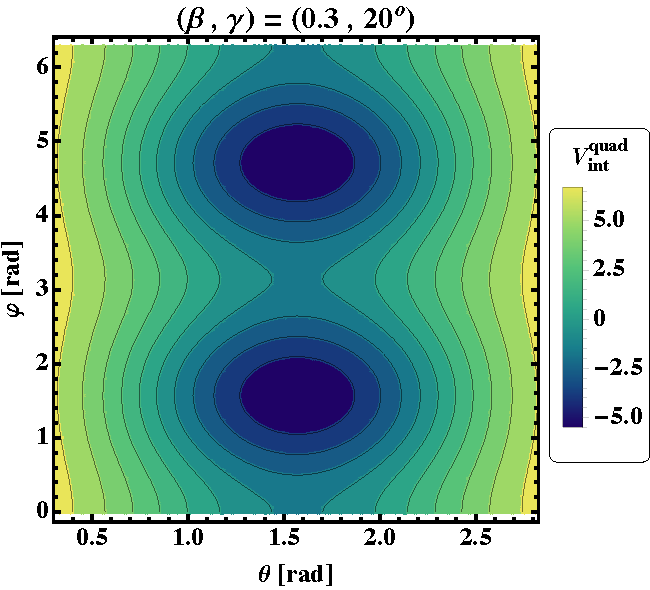
\includegraphics[scale=0.66]{Chapters/Figures/quadrupole-potentialV-2.pdf}
    \caption{The quadrupole potential $V_\text{int}^\text{quad}$ as defined in Eq. \ref{quadrupole-deformed-potential-V}, represented as a function of the angular coordinates $\theta$ and $\varphi$. Calculations were done with fixed parameters $\beta_2$, $\gamma$, and for $A=163$.}
    \label{figs-deformed-quadrupole-potential-1}
\end{figure}

\begin{figure}
    \centering
    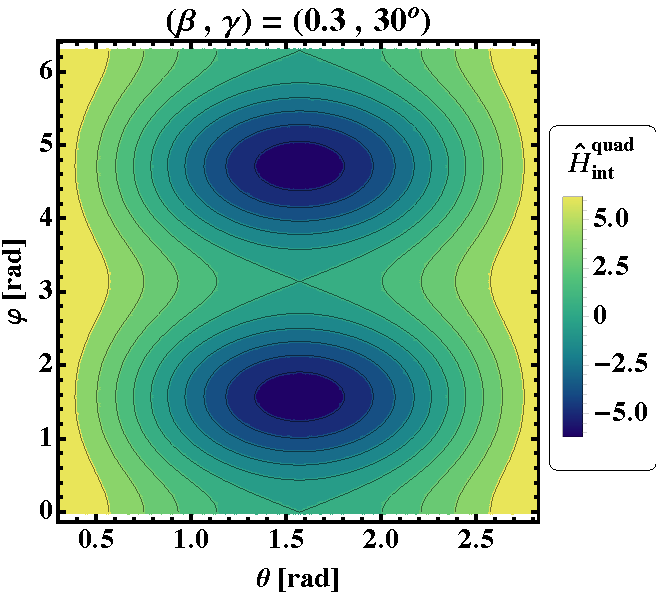
\includegraphics[scale=0.66]{Chapters/Figures/quadrupole-potentialV-3.pdf}
    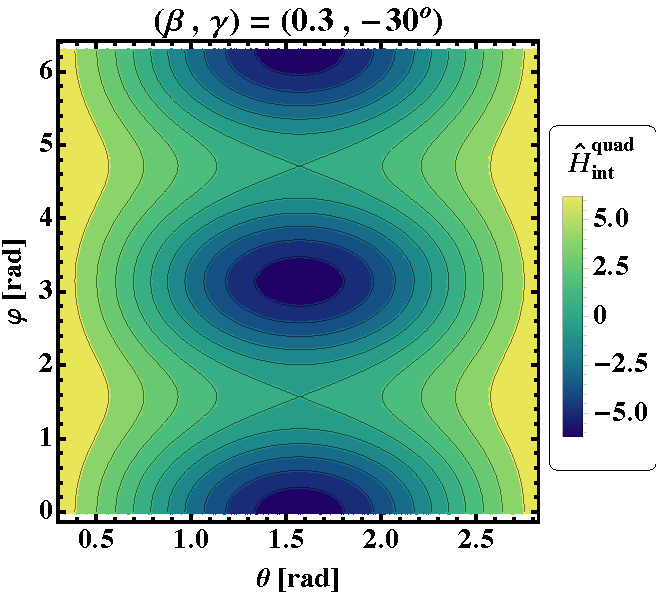
\includegraphics[scale=0.66]{Chapters/Figures/quadrupole-potentialV-4.pdf}
    \caption{The quadrupole potential $V_\text{int}^\text{quad}$ as defined in Eq. \ref{quadrupole-deformed-potential-V}, represented as a function of the angular coordinates $\theta$ and $\varphi$. Calculations were done with fixed parameters $\beta_2$, $\gamma$, and for $A=163$.}
    \label{figs-deformed-quadrupole-potential-2}
\end{figure}

For the evaluation of $h$, one can take the case when only the diagonal components of $h$ are considered and apply the rules only for one proton ($p$). As a result, the \emph{mixing terms} $j_+$ and $j_-$ from $h$ won't contribute at all, since their action on protonic states $\ket{jk}$ will give zero. Only the $(j_3^2-j(j+1)/3)$ term will contribute to the diagonal components of $h$. For a proton state $\ket{jk}$, where $k=-j,\dots,j$, the diagonal element $\bra{jk}h\ket{jk}$ will be:
\begin{align}
    h_{jk}\equiv\bra{jk}h\ket{jk}=\frac{1}{2}C_\beta\cos\gamma\bra{jk}\left(j_3^2-\frac{j(j+1)}{3}\right)\ket{jk}\ ,
\end{align}
which can be simplified to:
\begin{align}
    h_{jk}=\frac{1}{2}C_\beta\cos\gamma\left(k^2-\frac{j(j+1)}{3}\right)\ .
    \label{hdiag-equation}
\end{align}
This matrix elements will be functions of deformation parameters as well as the projection $k$ of the particle'
s angular momentum onto the $3$-axis. Since $j_3$ is applied twice on $\ket{jk}$ state, the final result will be $k^2$, so only the positive values can be considered for the numerical application $k=1/2,\dots,j$. When a high-$j$ proton orbital (say $h_{11/2}$ or $i_{13/2}$) is considered, for a nucleus with $A=167$, the evolution of $h_{jk}$ as function of $\beta_2$ and $\gamma$, respectively, are shown in Figs. \ref{hdiag-beta-evolution}. For completeness, the evolution w.r.t. the triaxiality parameter $\gamma$ for the diagonal matrix elements of $h$ are shown Fig. \ref{hdiag-gamma-evolution}.

\begin{figure}
    \centering
    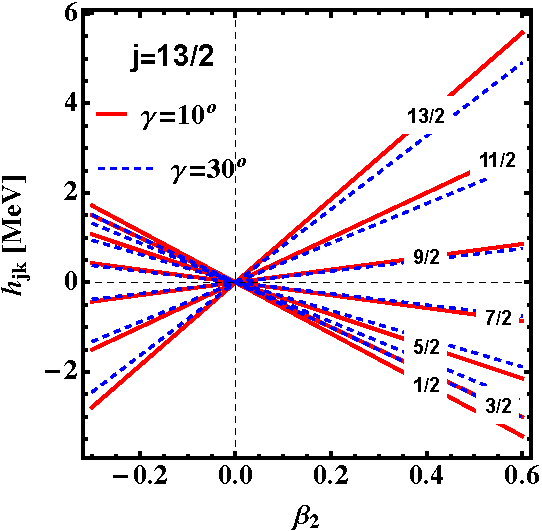
\includegraphics[scale=0.7]{Chapters/Figures/singleParticle-hdiag-1.pdf}
    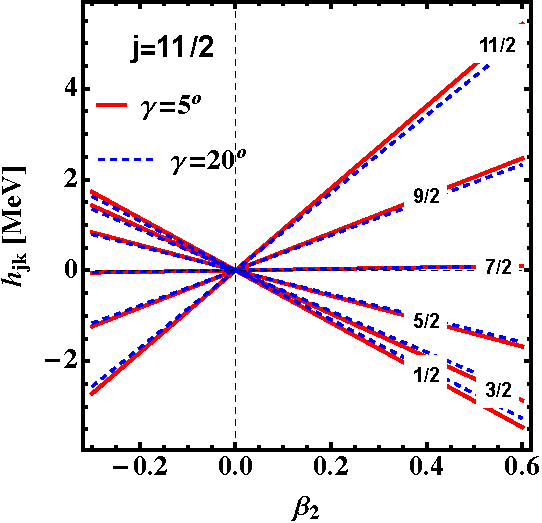
\includegraphics[scale=0.7]{Chapters/Figures/singleParticle-hdiag-2.pdf}
    \caption{The evolution with quadrupole deformation parameter $\beta_2$ for the diagonal matrix elements of $h_{jk}$ defined in Eq. \ref{hdiag-equation} (proton on a defined $j$-shell), at a fixed triaxiality parameter $\gamma$. See text for details.}
    \label{hdiag-beta-evolution}
\end{figure}

\begin{figure}
    \centering
    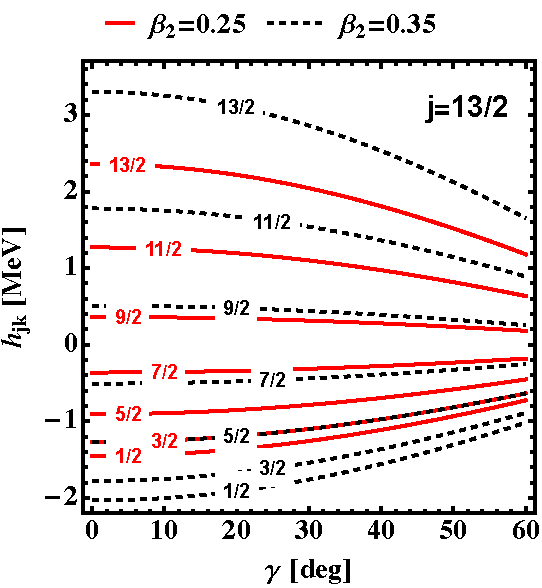
\includegraphics[scale=0.7]{Chapters/Figures/hdiag-gamma-1.pdf}
    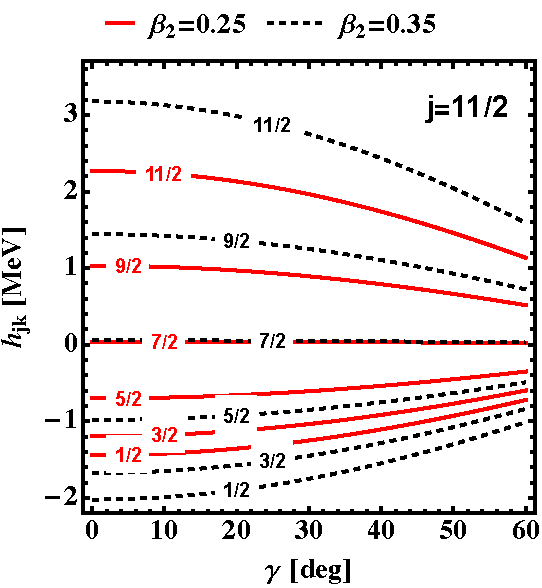
\includegraphics[scale=0.7]{Chapters/Figures/hdiag-gamma-2.pdf}
    \caption{The evolution with triaxiality parameter $\gamma$ for the diagonal matrix elements of $h_{jk}$ defined in Eq. \ref{hdiag-equation} (proton on a defined $j$-shell), at a fixed deformation parameter $\beta_2$. See text for details.}
    \label{hdiag-gamma-evolution}
\end{figure}

Regarding this numerical application, one can observe the fact that since only the cosine function is present in the diagonal components of $h$, the single-particle energies are independent on the sign of $\gamma$ (since cosine is an even function). However, this is not the case when calculations are done for the non-diagonal elements, since states with different $k$ will add contributions to $h$ via the sine function. For the evolution of $h_{jk}$ with $\beta_2$, one can see that the lines in Fig. \ref{hdiag-beta-evolution} (especially the right plot) are almost similar, indicating that the diagonal components are not very sensitive to nuclear triaxiality. On the other hand, a difference in $\beta_2$ between the components will result in large gaps.

Concluding this section, by using the triaxial PRM one can describe the energies of a an odd-$A$ triaxial nucleus, and moreover, as it will be shown, quantities such as transition probabilities (electric quadrupole type) and quadrupole moments can be calculated. It is a starting ground for multiple theoretical descriptions which aim to verify, confirm, and even predict phenomena specific to highly deformed shapes.

\section{Stable Triaxial Deformation}

As it was mentioned, across the chart of nuclides, stable isotopes do exist in an \emph{equilibrium} at which no symmetries are involved with regards to their shape. Quantitatively, the stability of a triaxial nucleus is related to the presence (existence) of minima within the \emph{Potential Energy Surface}. This energy surface characterizes the shape of the nuclear surface with respect to the deformation parameters $\beta$ and $\gamma$. One can speculate on the fact that for an ellipsoidal shape, the total energy at a fixed angular momentum, function of the deformation will be given as \cite{ring2004nuclear}:
\begin{align}
    E(\beta,\gamma,I)=E_\text{LDM}(\beta,\gamma,I)+E_\text{shell}(\beta,\gamma,I)-\bar{E}_\text{corr}(\beta,\gamma,I)\ ,
    \label{energy-surface-correction-terms}
\end{align}
where $E_\text{LDM}$ is the deformation energy for a rotating ellipsoid (characterized by the rigid-like MOI, since at high spin values this approximation holds true), $E_\text{shell}$ is the energy within the shell model (can even use the Nilsson's deformed variant), and $\bar{E}_\text{corr}$ is usually calculated as an \emph{averaged value} of the Nilsson-Strutinsky corrected potential \cite{brack1972funny} (which is beyond the scope of this work). Finding these energies can be done by working at constant $\omega$ or at constant I, when diagonalizing the deformed-single particle potential in the rotating frame \cite{ring2004nuclear}.

Solving thus Eq. \ref{energy-surface-correction-terms} results in having a \emph{qualitative} analysis for the behavior of the nucleonic matter at high spins. These `solutions' will consist of graphical representations in the $(\beta,\gamma)$-plane, where values with different magnitudes for the potential energy appear. The lower these values are, the `more stable' the deformation is. Typically, one can find regions of stability across the plane with well-defined values for $\beta$ and $\gamma$ at which nucleus is stable and deformed. On the other hand, if the energy variation is rather flat in the $\gamma$ degree of freedom, but centered around a finite $\beta$, then this nucleus is called \emph{$\gamma$-unstable}. These energy surfaces are a key indicator of stability with respect to the deformation parameters. Examples of energy surfaces for some nuclei are shown in Figs. \ref{pes-example-set-1}. It is remarkable the fact that small quantum fluctuations will exist around the minima.
In order to explain the theoretical implications of Figs. \ref{pes-example-set-1}, one needs to understand that based on a MHO, a so-called \emph{Ultimate Cranker} (UC) numerical implementation has been developed \cite{bengtsson1989method,bengtsson1990high} (a Nilsson deformed potential in which pairing interaction is taken into account). This implementation is able to give the values for $(\beta,\gamma)$ at which a nucleus might achieve stability, practically identifying local and global minima within the potential energy surface. In a future section, multiple isotopes with known stable triaxiality will be classified in terms of the deformation parameters, creating thus an `inventory' with these deformed nuclei.

\begin{figure}
    \centering
    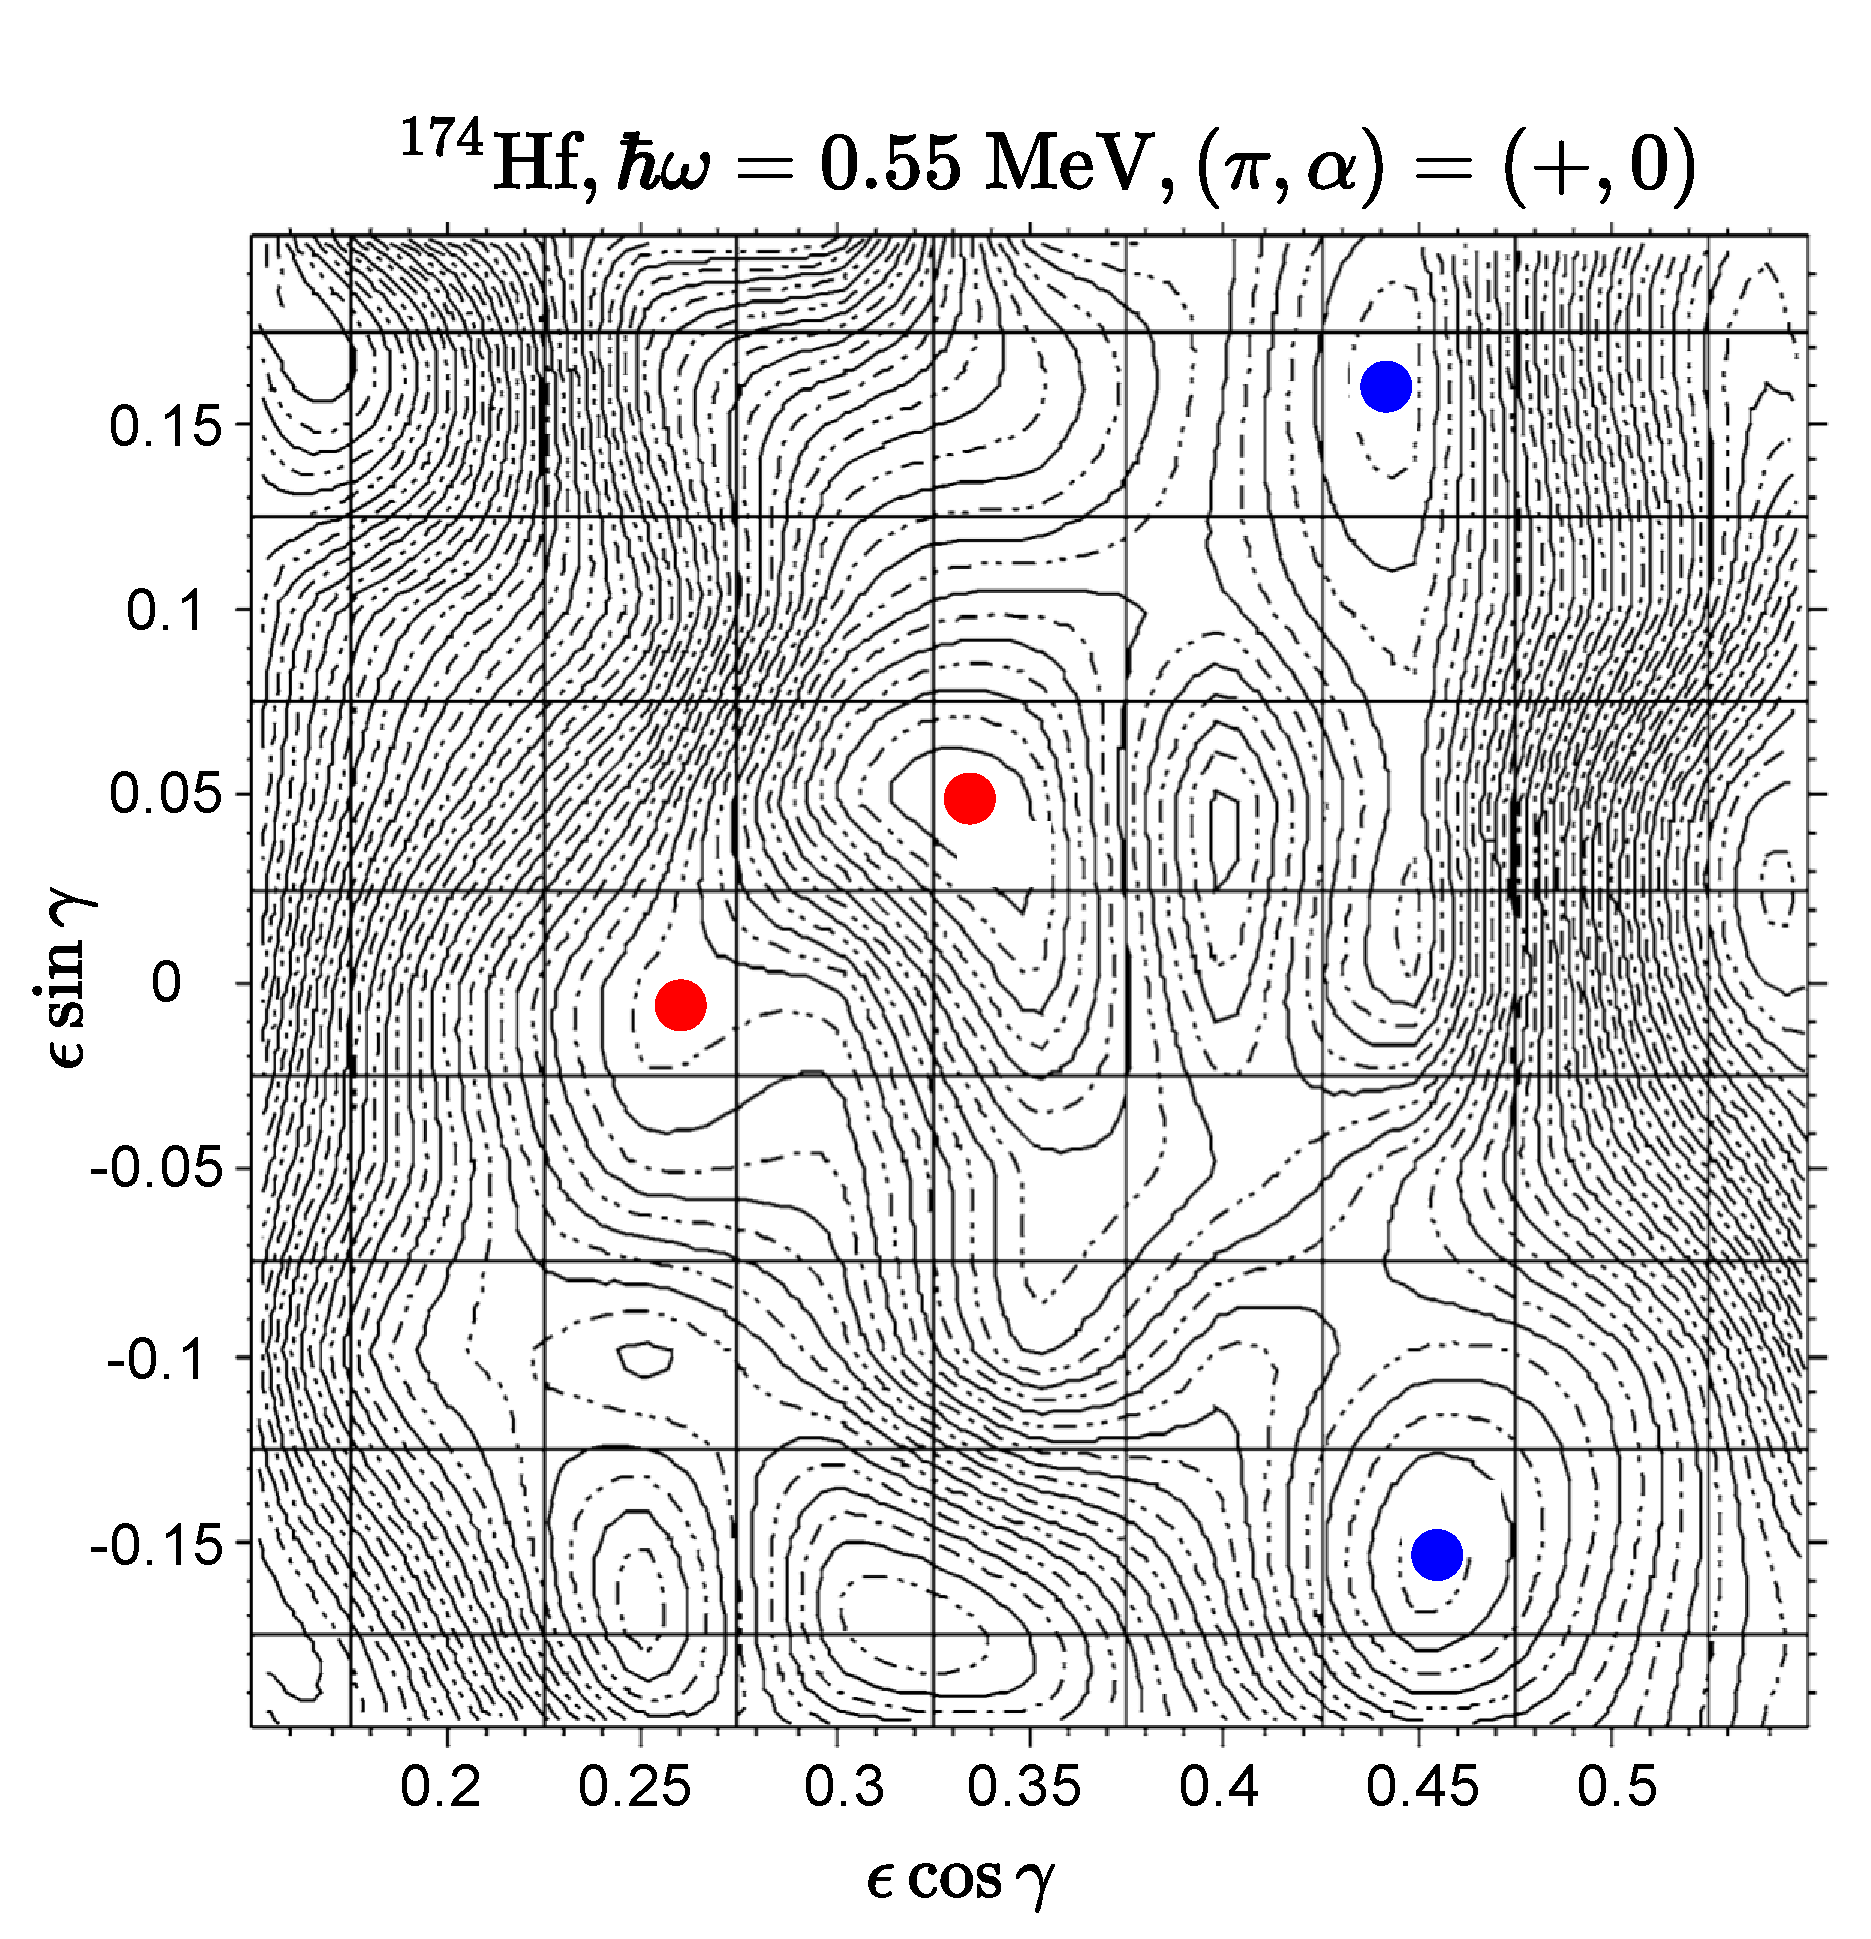
\includegraphics[width=0.49\textwidth]{Chapters/Figures/174Hf-PES.pdf}
    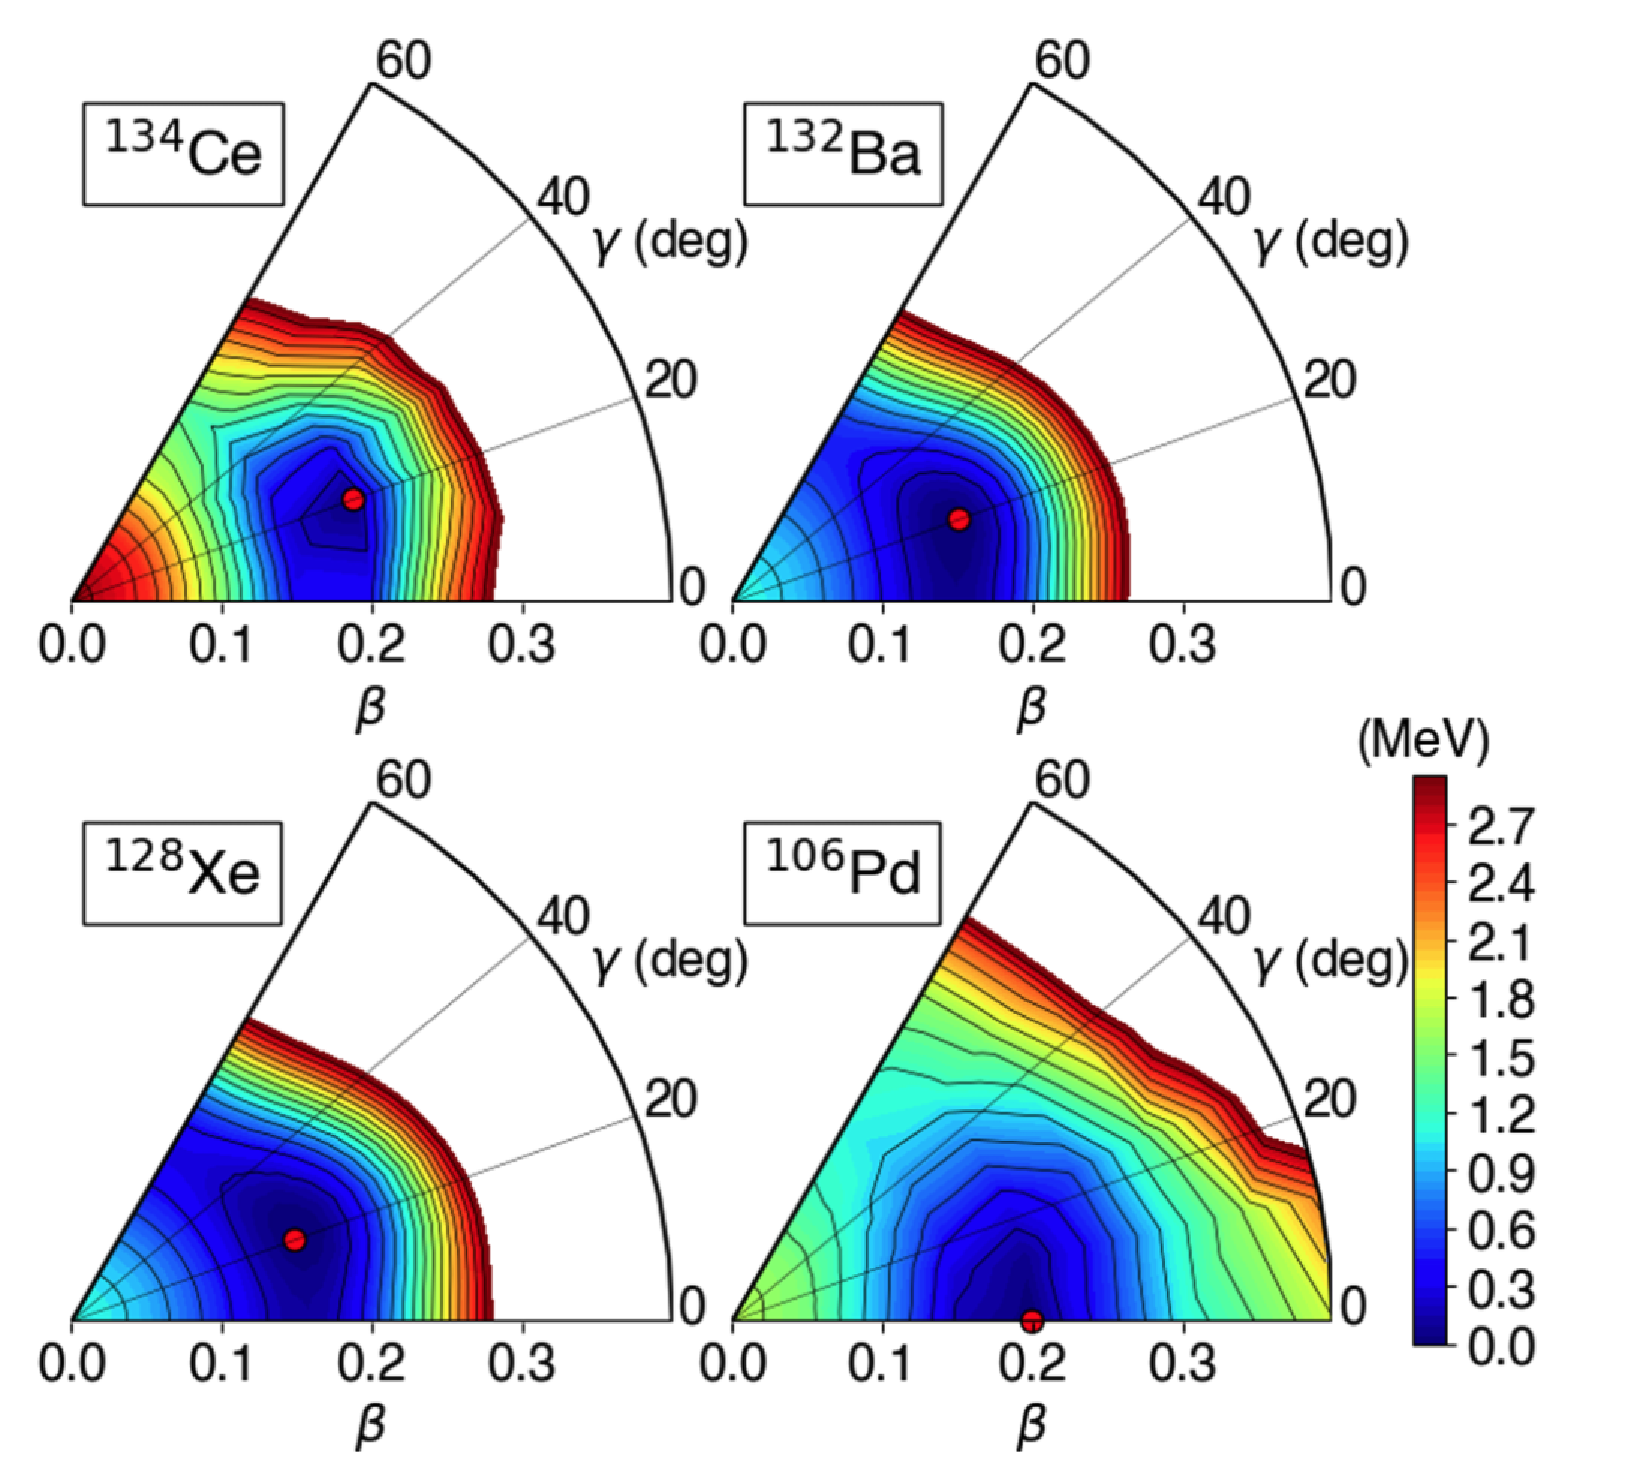
\includegraphics[width=0.49\textwidth]{Chapters/Figures/even-A-PES.pdf}
    \caption{\textbf{Left:} Potential energy surface for $^{174}$Hf, evaluated at a constant rotational frequency. Positive parity and a signature $\alpha=0$ were considered. Four minima that could be attributed to known configurations are identified which are marked with red colored dots (normal deformation) and blue dots (strong deformation). This figure was taken from Ref. \cite{djongolov2003extending}. \textbf{Right:} PES for some even-even nuclei.}
    \label{pes-example-set-1}
\end{figure}

This figure was taken from Ref. \cite{nomura2021examining}. Note the rather shallow triaxial minima for all nuclei, and the $\gamma$-soft nature of all the nuclei except for, whose minimum is achieved at a null triaxiality parameter.

\section{Fingerprints of Triaxiality}